Recently, a superpisition of hype and hope has been put on the  %~\cite{preskill2018quantum, peruzzo2014variational, pesah2021absense,sharma2022reformulation,biamonte2017quantum
field of quantum machine learning~\cite{biamonte2017quantum, supremacygoogle, schuld2021isquantum, Aaronson2015, preskill2018quantum, peruzzo2014variational, pesah2021absense,sharma2022reformulation}, particularly when \textit{training} Parametrized Quantum Circuits (PQCs).

PQCs consists on a series of quantum gates, \textit{e.g.} CNOTs and rotations, where the real parameters of the latter are modified in order to \textit{optimize} the circuit. Here, and in analogy to the classical neural networks scenario~\cite{Goodfellow-et-al-2016}, we aim to minimize a given cost function (and thereby, these circuits are also known as \textit{quantum neural networks}). The overall training of PQCs is known as a Variational Quantum Algorithm (VQA), and consists on an hybdrid classical-quantum scheme. In turn, a quantum device is only used to estimate cost-function values, whereas a classical algortihm is in charge of controlling that quantum device by optimizing over accessible degrees of freedom, \textit{e.g.} rotation parameter values. Recently, many efforts have been carried out in order to analyze the performance, trainability and overall feasibility of VQAs~\cite{VQA_revmarco, VQA_revalba}.

Training a VQA means to solve an optimization problem encoded into a cost function of the form
\begin{equation}\label{eq:cost}
    C(\kvec,\thv)=\sum_i^M f_i\left(\tr{\Oi U(\kvec,\thv)\rho_i U^\dagger (\kvec,\thv)}\right)  \,.
\end{equation}
Here, $\{\rho_i\}$ are $n$-qubit states forming a \textit{training set} of cardinality $M$, and $U(\kvec,\thv)$ is our NISQ circuit parametrized by continuous parameters $\thv$ (\textit{e.g.}, rotation angles) and by discrete parameters $\kvec$ (\textit{e.g.}, gate placements). Moreover, $\Oi$ are observables and $f_i$ are functions that encode the optimization task at hand.

For example, when employing the Variational Quantum Eigensolver (VQE) algorithm~\cite{peruzzo2014variational} we have $f_i(x)=x$ and the cost function reduces to
\eq{vqe_cost}{C_{\text{VQE}}(\kvec,\thv)=\tr{\hat{H} U(\kvec,\thv)\rho U^\dagger (\kvec,\thv)},}where $\rho$ is the input state (and the only state in the training set) and $H$ is the Hamiltonian whose ground state we seek to prepare. Alternatively, in a classification problem where the training set is of the form $\{\rho_i,y_i\}$, with $y_i\in \{1,...,n\}$ being the true label, the choice $f_i(x)=(x-y_i)^2$ leads to the least square error cost~\cite{classiVQA, vqaclass1, vqaclass2,vqaclass4, cong2019quantum}.
In this regard, and as it happens in the reinforcement-learning scenario discussed in Sec.~\ref{sec:1_rl}, the possibility of encoding a given problem into a cost function is a matter of creativity.

\vspace{1cm}

Given the cost function, a NISQ circuit is employed to estimate each term in Eq.~\eqref{eq:cost}. Ussually, the available measurements consist on local projections over the eigenbasis of $\sigma^{i}_z$ for each qubit $i=1,...,n$. Here, in order to estimate the cost function, we decompose each operator appearing in the cost-function in terms of \textit{Pauli-strings}. Recall that Pauli-string operators form a basis in the space of $n$-dimensional hermitian operators and hence
\eq{decoH}{ \Oi = \sum_{k=1}^{4^n} c_k P_k,}
with $P_k = \bigotimes_{i=1}^n\mathbb{\sigma}_j$, where $\mathbb{\sigma}_j \in \llaves{\mathbb{I}, \sigma_x, \sigma_y, \sigma_z}$. Note that Pauli-string operators are orthogonal to each other, \textit{i.e.} $\tr{P_k P_{k'}} = 2^n \delta_{k k'}$ and thus $c_k = \tr{\Oi P_k}/2^n$.

Thus, the cost-function can be estimated by computing averages of some pre-determined observables, which are in turn a weighted sum of expected values of Pauli-strings. Moreover, we can estimate each expected value $\langle P_k\rangle$ by performing the corresponding single-qubit transformation beforehand and measuring $\sigma_z$\footnote{This can be understood as a change-of-basis.}. In this regard, if an $\epsilon$-accuracy is required in order to estimate this expected value, an order of $\sim \frac{1}{\epsilon^2}$ measurements needs to be done (this will have consequences when trying to resolve between very small values of the cost-function in Sec.~\ref{ssec:1_nisq_barrenplateaus}).

We also note that the Pauli-string procedure outlined above consists on an exponentially large sum of expected values. However, we are often interested in local hamiltonians, where many of these terms vanish (for example, TFIM and XXZ models considered in Ch.~\ref{chapter:VANS}). In this case, techniques such as randomized measurements (RMs) have recently been developed, in which the cost function can be computed more efficiently. While we do not consider such approaches in this thesis, we refer the interested reader to Ref.~\cite{elben2022randomized}, and we note that a combination between our methods (discussed in Chapter~\ref{chapter:VANS}) and classical shadows (a sub-class of RMs) is discussed in Sec.~\ref{ssec:vans_discu}.

\vspace{1cm}

Once the cost-function has been estimated, the power of classical optimization algorithms is leveraged to solve the optimization task
\begin{equation}\label{eq:optimization}
    \argmin{\kvec,\thv} C(\kvec,\thv)\,.
\end{equation}
\begin{figure}[t!]
    \centering
    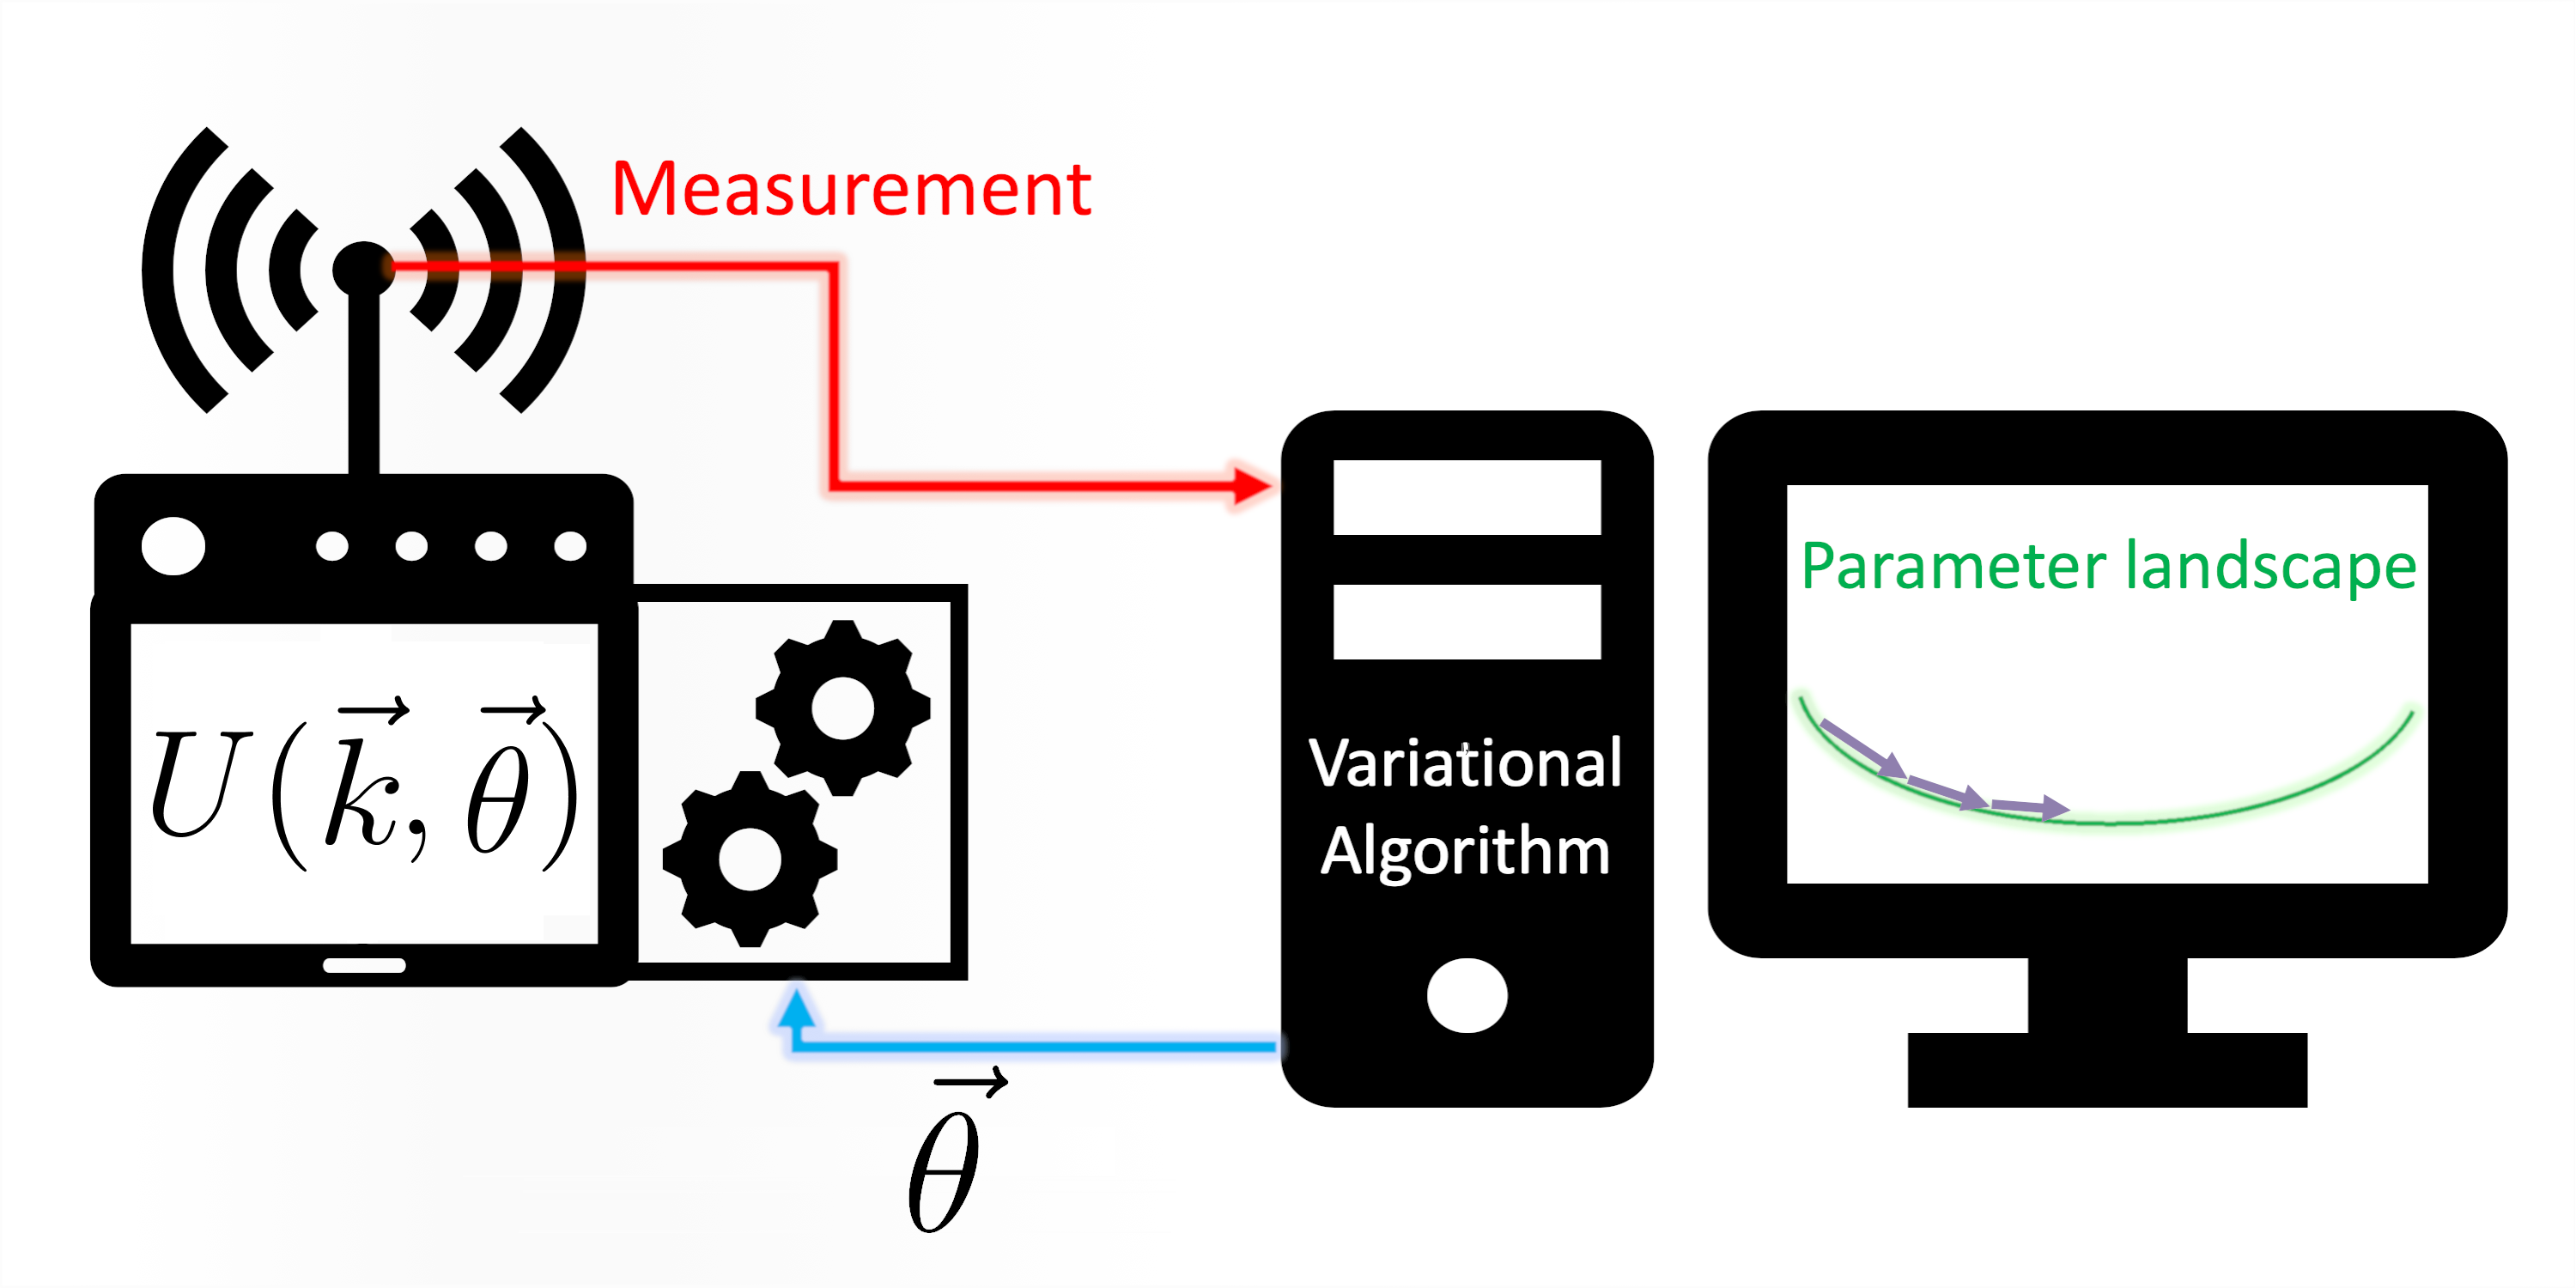
\includegraphics[width=1.\textwidth]{Figures/VANS/vqa_cycle.png}
    \caption{Figure adapted from Ref.~\cite{borrowed}: a generic VQA algortihm is sketched. Here, a quantum device is used to estimate a cost-function value, whereas the device itself is controlled by a classical optimization algorithm. This cycle is iterated until convergence.}
    \label{fig:VQAcycle}
\end{figure}
The estimation of a cost function via a quantum circuit and its modification (hopefully towards a cost-minimizing direction) by a classical optimization algorithm defines a cycle, which is repeated until convergence, as depicted in Fig.~\ref{fig:VQAcycle}. The success of such scheme hinges on several factors. As a matter of fact, the classical optimizer must be able to efficiently train the parameters, and in the past few years, there has been a tremendous effort in developing quantum-aware optimizers~\cite{verdon2018universal,kubler2020adaptive,arrasmith2020operator,stokes2020quantum,koczor2019quantum,nakanishi2020sequential,fontana2020optimizing}. In particular, severe trainability issues has been pointed out, which forbid the success of VQAs and as constitute the main barrer (along with hardware-noise) for making use of current NISQ devices in the VQA framework, and we will review some of them in Sec.~\ref{ssec:1_nisq_vans_bp}.

However, we note that even if such trainability issues could be overcomed, the performance of a VQA will intrinsically be linked to the specific quantum circuit used for the training. Here, the choice of an ansatz for $U(\kvec,\thv)$ plays a crucial role in determining the success of a VQA scheme; for instance, for a given Hamiltonian in the VQE algorithm, circuits that are close to the ground-state preparing one might lie outside the subspace $\mathcal{U}$ of the unitary group $U(n)$ which is generated by varying $\thv$ in $U(\kvec, \thv)$, with a fixed circuit layout given by $\kvec$~\cite{holmes2021connecting}.

In this respect, not every unitary transformation in $U(n)$ can straightforwardly be implemented, since the availability of quantum gates is often restricted; we generally need to deal with a \textit{gate-dictionary} $\mathcal{D}$, which in this thesis will be composed of one-qubit rotations and of CNOTs entangling any pair of qubits present in the circuit. We note that such an dictionary is universal~\cite{nielsen00}: any quantum gate can be implemented provided enough gates of the dictionary are used. Nevertheless, such a \textit{compilation} is a tricky one: noise accumulates with circuit's depth, and hence only a non-trivial set of unitaries can be reached. Moreover, we remark that the availability of fully-connected qubits is a slight simplification, and connectivity constraints should in principle be considered. In the latter case, entangling two qubits which are not straightforwardly connected represents an overhead in circuit's depth, and many efforts have been carried out recently in order to find novel strategies to tackle this issue~\cite{compilingDeepRLmaster}.

For these reasons, it is important to discuss different strategies ussually considered when constructing the quantum-circuit to be used in a VQA, also known as an \textit{ansatz}. %Here, we can readily distinguish between fixed-structure quantum circuits (where only the continuous paramters encoded in the rotations values are optimized), and variable-structure ones, in which both parameters \textit{and} strucure are optimized.
